\chapter{Classifying Tables Describing Comparisons}
\label{table_classification}
A lot of valuable information about comparisons with some baselines and other research is present in the tables of academic research. Researchers tend to spend much valuable time finding the citations and the table of results from those citations. Sci-Genie via Citation Graph and the Machine Learning models helps filter tables describing comparisons at the time of reading research. 

This chapter will cover classifying tables that describe a comparison of entities and propose approaches to tackle the problem of classifying such types of tables. 

\section{Problem Formulation}

The structure of the tables in scientific research can fluctuate based on the information presented by the tables. The tables may also contain information whose context cannot be exactly inferred without the caption underneath the table. Tables occurring in scientific research can also be segregated into well-defined types such as the ones described in Chapter \ref{relatedwork:table-type}. These tables may also not contain a directly linkable entity from a knowledge base(KB) as entities defined in the research may not be present in the KB. Due to such different intrinsic characteristics, models trained using knowledge bases along with web tables such as the one by \cite{deng2020turl} cannot be directly fit to solve this problem. 

\begin{table}
    \label{table\arabic{tablecounter}}
    \centering
    \begin{tabular}{|l|l|l|}
        \hline
        Symbol & Meaning & Type \\ \hline
        $Y$ & Labels & Discrete : $\{0,1\}$ \\ \hline
        $X_T$ & Cell Embedding & $\mathbb{R}^{T_l \times d}$\\ \hline
        $X_C$ & Caption Embedding & $\mathbb{R}^{C_l \times d}$ \\ \hline
        $P_C$ & Positional Embedding & $\mathbb{R}^{C_l \times d}$ \\ \hline
        $E_r$ & Row Embedding & $\mathbb{R}^{T_l \times d}$ \\ \hline
        $E_c$ & Column Embedding & $\mathbb{R}^{T_l \times d}$ \\ \hline
        $T_l$ & Number Of Cells & $\mathbb{N}$ \\ \hline
        $T_r$ & Number Of Rows & $\mathbb{N}$ \\ \hline
        $T_c$ & Number Of Columns & $\mathbb{N}$ \\ \hline
        $C_l$ & Length of Caption & $\mathbb{N}$ \\ \hline
        $T_{cell}$ & Sequnces of Cells & $\mathbb{N}^{T_l}$ \\ \hline
        $f_\theta$ & Neural Network & - \\ \hline
    \end{tabular}
    \caption{\label{tablecounter} Table Of Symbols for Equations}
\end{table}
\refstepcounter{tablecounter}
The problem of classifying a table $T$ as a table describing a comparison can be framed as a binary classification problem. Given a table $T$ and its caption $C$, the classifier $f_\theta(T,C) \rightarrow Y$ predicts a binary label $Y \in \{0,1\}$ to denote weather the table is describing a comparison of entities\footnote{Both the table and caption are used because human labeling discovered that these two variables are the most prominant indicators of a table describing a comparison.}. 

Based on this formulation, this dissertation analyzes 4 different types of ML models and the representations they use for the table $T$ and caption $C$ for the problem:
\begin{itemize}
    \item Cross Channel Transformers With/Without Pretraining
    \item Encoder Only Multi-Channel Transformer With Pretraining
    \item Finetuning Pretrained Scibert
    \item SVM and Naive Bayes (Baselines)
\end{itemize}

Different models are analyzed because the representations of $T$ and $C$ can be treated as seperate variables or as a single variable based on the model. Cross Channel Transformer, Encoder Only Multi-Channel Transformer treats $T$ and $C$ as seperate representations, Scibert, SVM and Naive Bayes treats $T$ and $C$ as one joint representation. 

Section \ref{table_classification:models} describes the models developed/trained for the input representations of table $T$ and caption $C$. The data collection and labeling for the machine learning models is described in Section \ref{table_classification:data-coll}. The experiment results for different models is described in Section \ref{table_classification:experiement-result}

\section{Classification Models}
\label{table_classification:models}

\subsection{Encoder Only Multi-Channel Transformer}
\label{table_classification:models:encoder-model}
\begin{figure}[h]
    \centering
    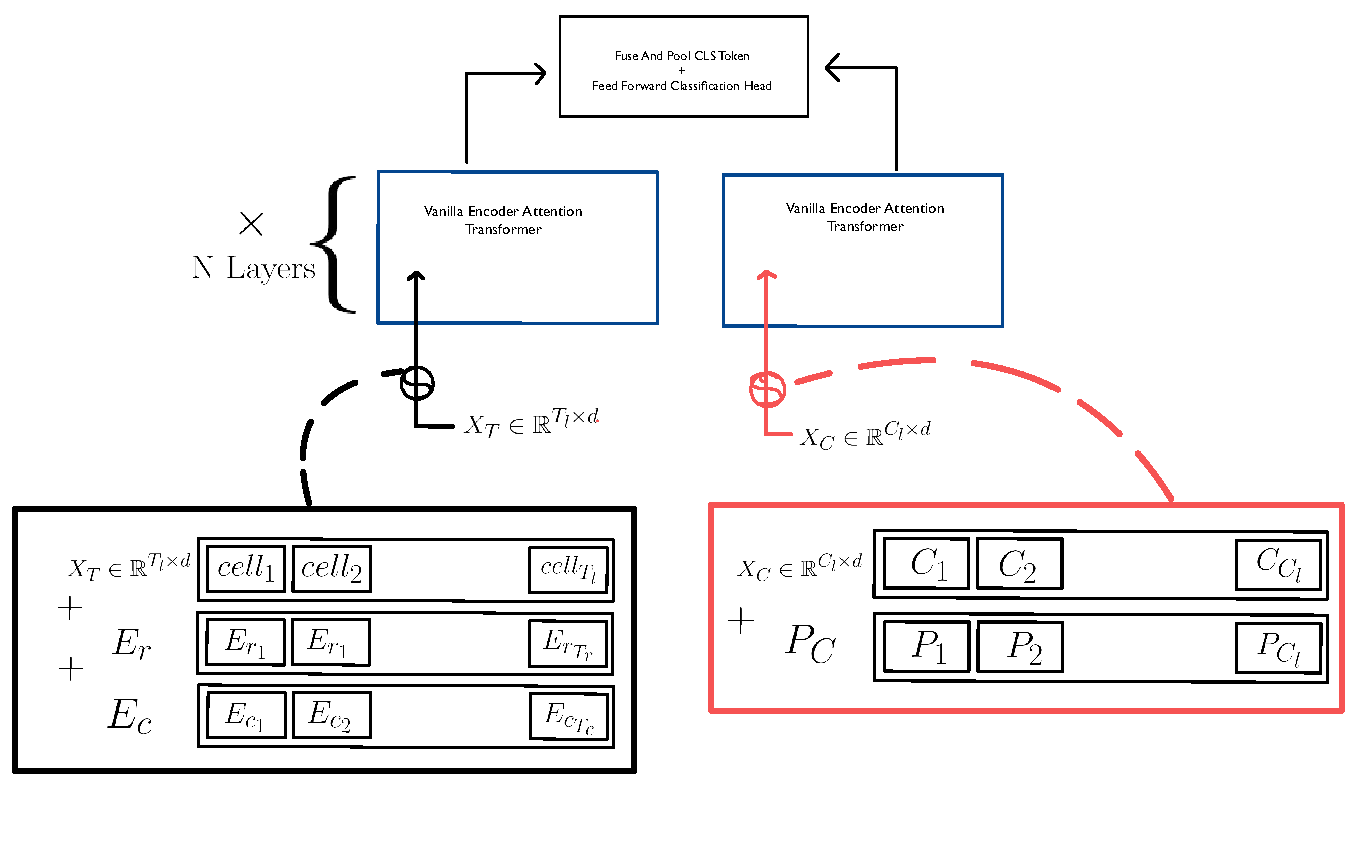
\includegraphics[width=\maxwidth{\textwidth}]{src/images/tabmod-enconly.pdf}
    \caption{Encoder Attention Transformer For Table Classification}
    \label{figure\arabic{figurecounter}}
\end{figure}
\refstepcounter{figurecounter}
Based on the models developed by \cite{deng2020turl}. A structurally-aware encoder only Transformer model is adapted to fit the function $f_\theta$. Figure \ref{figure17} visualises the model and its input representations.

\subsubsection{Input Representation}
\label{table_classification:models:encoder-model:input-rep}
Each table $T$ is represented as tuple of $(T_{cell},E_r,E_c)$; where $T_{cell} \in \mathbb{N}^{T_l}$ are the cells of the table represented as a sequence of integer tokens; $E_r$ is the row embedding where embedding $E_{r_{i}}$ represents the row of the cell $T_{cell_{i}}$ as an embedding;  $E_c$ is the column embedding where an embedding $E_{c_{i}}$ represents the column of the cell $T_{cell_{i}}$ as an embedding. The caption $C$ is represented as sequence of integer tokens which will be transformed to embeddings by the Transformer Model. The representations for the table $T$ are inspired from the models created by \cite{deng2020turl}. 

The cell sequence tokens $T_{cell}$ and caption $C$ are created using a word-piece tokenizer from the SciBert Model \footnote{https://huggingface.co/allenai/scibert\_scivocab\_uncased}. The tokenizer converts the value of individual cells or the caption into a sequence of integer tokens. These tokens can be used to create embeddings which are passed to the transformer model. 

\subsubsection{Model Description}
The table cell sequence $T_{cell}$ and the Caption $C$ are first converted to embeddings $X_T, X_C$ respectively. Post creation of the embeddings, the caption embedding  $X_C$ is added with the position embedding $P_C$; The cell embeddings $X_T$ are added with $E_r,E_c$. After the additions of the respective embeddings, differentiable CLS tokens are concatenated to $X_T,X_C$.

These embeddings are passed to individual encoder self-attention transformers. The class tokens from the final layer is pooled and sent for classification using a linear feed forward layer and a cross entropy loss is applied on the predictions. Figure \ref{figure17} visualizes the model. 


\subsection{Cross Channel Transformer}
\label{table_classification:models:cross-channel}
\begin{figure}[h]
    \centering
    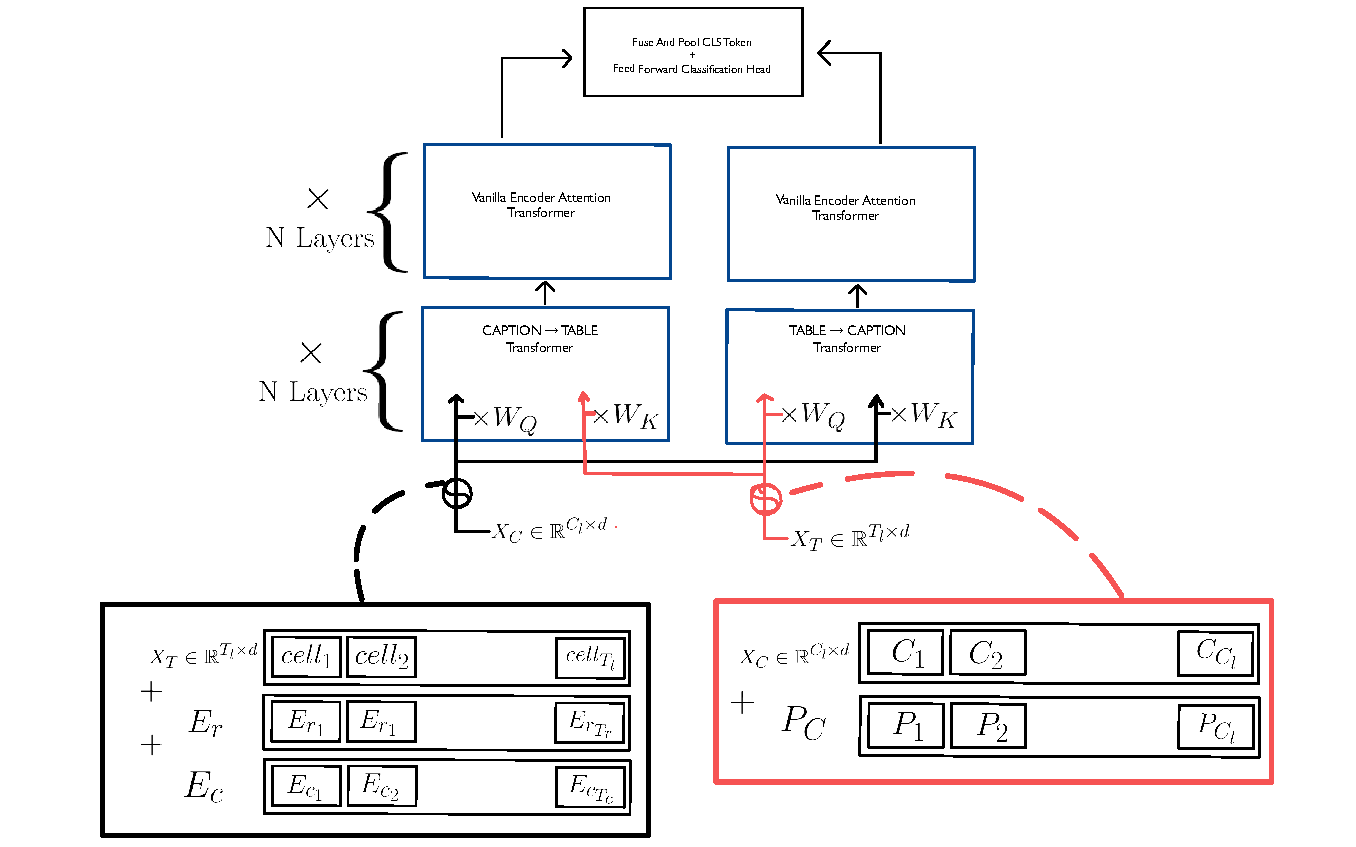
\includegraphics[width=\maxwidth{\textwidth}]{src/images/tablemodel.pdf}
    \caption{Cross Channel Transformer For Table Classification}
    \label{figure\arabic{figurecounter}}
\end{figure}
\refstepcounter{figurecounter}

Based on the models developed by \cite{tsai2019multimodal} and \cite{deng2020turl}, a structurally-aware cross channel Transformer model is adapted to fit the function $f_\theta$. Figure \ref{figure18} shows the outline of the model. This model is chosen to validate wheather cross attention will have an influence on the performance of the model if intermediate presentations for Table $T$ and Caption $C$ are generated from the cross attention operation. 

\subsubsection{Input Representation}
The input representations for $T$ and $C$ are the same as given in Section \ref{table_classification:models:encoder-model:input-rep}


\subsubsection{Model Description}
The table cell sequence $T_{cell}$ and the Caption $C$ are first converted to embeddings $X_T, X_C$ respectively. Post creation of the embeddings,  the caption embedding  $X_C$ is added with the position embedding $P_C$; The cell embeddings $X_T$ are added with $E_r,E_c$. After the additions of the respective embeddings, differentiable CLS tokens are concatenated to $X_T,X_C$.
These embeddings are passed to separate cross channel attention transformer layers \parencite{tsai2019multimodal} after which they are passed to the vanilla transformer encoder attention layers \parencite{vaswani2017attention}. Different strategies are chosen for handling the output of the vanilla tranformer encoder based on the type of task. 

Embeddings at the CLS token position, are pooled from the sequences and concatenated for the table of comparison classification task. Once concatenated, this joint embedding is passed to feed forward layers for classification using Cross Entropy Loss. For the pretaining task, the last vanilla encoder layer’s output will be used for predicting the masked tokens of the input table cells $T_{cell}$ and the caption $C$.

\subsection{Finetuning Scibert Transformer Model}
\cite{beltagy2019scibert} created a model which was trained on large full text corpus of scientific research containing 1.14M research papers. As this model has been subjected large amounts of pretraining, it is chosen for fine tuning for the same problem as the model may have encountered data of a similar distribution. 
\subsubsection{Input Representation}
\label{table_classification:models:sb:input_rep}
For the finetuning of SciBert, The Table $T$ and caption $C$ are serialized to strings and one concatenated string is created. An example representation is given below: 
\begin{verbatim}
    CAPTION : Table 1: Feature extraction time (Seconds), 
    number of parameters (Millions), and network size (Megabytes) 
    for each source on Office + Caltech-10 datasets.

    TABLE :                          0         1           2      3
0                     Task  Net size  Parameters   Time
1          Squeezenet [17]        46        1.24   13.3
2             Alexnet [21]       227          61   13.9
3           Googlenet [40]        27           7   15.9
4          Shufflenet [51]       6.3         1.4   17.0
5            Resnet18 [15]        44        11.7   14.8
6               Vgg16 [36]       515         138   33.6
7               Vgg19 [36]       535         144   37.1
8         Mobilenetv2 [35]        13         3.5   21.4
9        Nasnetmobile [55]        20         5.3   39.3
10           Resnet50 [15]        96        25.6   22.7
11          Resnet101 [15]       167        44.6   26.7
12        Densenet201 [16]        77          20   61.8
13        Inceptionv3 [41]        89        23.9   28.2
14            Xception [4]        85        22.9   48.1
15  Inceptionresnetv2 [39]       209        55.9   54.1
16        Nasnetlarge [55]       360        88.9  141.2
\end{verbatim}

\subsubsection{Model Description}
The input representation string is converted to a sequence of integer tokens which are capped to the length of 512 tokens because of SciBert's constraint on maximum sequence length. A class token is added at the start of the sequence; the sequence is then passed to the Scibert Model. The class token is pooled from after the final layer and is passed to a feed forward neural network for binary classification using cross entropy loss. 


\subsubsection{Model Training}
The model is trained using the for 6 epochs with a linear learning rate warm up schedule of 20 epochs.

\subsection{Baselines}
SVM models are used as baselines as when \cite{kim2012scientific} conducted a study for table type classification, deep learning was not as popular. Naive Bayes(NB) model are also chosen as an additional baseline for the classification task. 

\subsubsection{Input Representation}
The input representation for the SVM and the NB model are the same as the string described in Section \ref{table_classification:models:sb:input_rep}. The string undergoes tokenisation and a classifier is trained based on TF/IDF values of the input strings. 

\subsection{Pretraining Transformers}
\label{table_classification:models:encoder-model:pre-train}
Based on the insights learned from \cite{hernandez2021scaling} on the effectiveness of pretrained models for downstream tasks, the cross-channel transformer model is pretrained with 70K tables from papers from ArXiv. A masked language modeling pretraining objective is used to train the Transformer model given in Figure \ref{figure18}, and \ref{figure17}. The pretraining follows the procedures described by \cite{deng2020turl} where the task is of Mask Language Modeling(MLM) for the sequence of cells $T_{cell}$ and the caption $C$. The model is tasked to predict the word token where a MASK token is inserted in the table $T$ and caption $C$. A mask is inserted in 80\% of the training samples with 15\% of the sequence being masked. The cross entropy losses from MLM predictions of the Table and Caption is added and backpropagated. 

This objective allows training the model with large number of tables instead of using classifiers trained on small amounts of data. The pretraining task is run for 35K steps in 5 epochs. The learning rate is set to 0.0001 for the pretraining task with an AdamW optimizer. Both the transformer models described in Section \ref{table_classification:models:encoder-model}, \ref{table_classification:models:cross-channel} are pretrained using the same MLM objective. 

\subsection{Finetuning Transformers}
After the Cross Channel Transformer and the Encoder Only Multi-Channel Transformer undergo the pretrainig task; the models are finetuned on the classification task with a learning rate of 2e-05, scheduled with a linear learning rate scheduler for 20 epochs using the AdamW optimizer. 

\section{Data Collection And Labeling}
\label{table_classification:data-coll}

\begin{figure}[h]
    \centering
    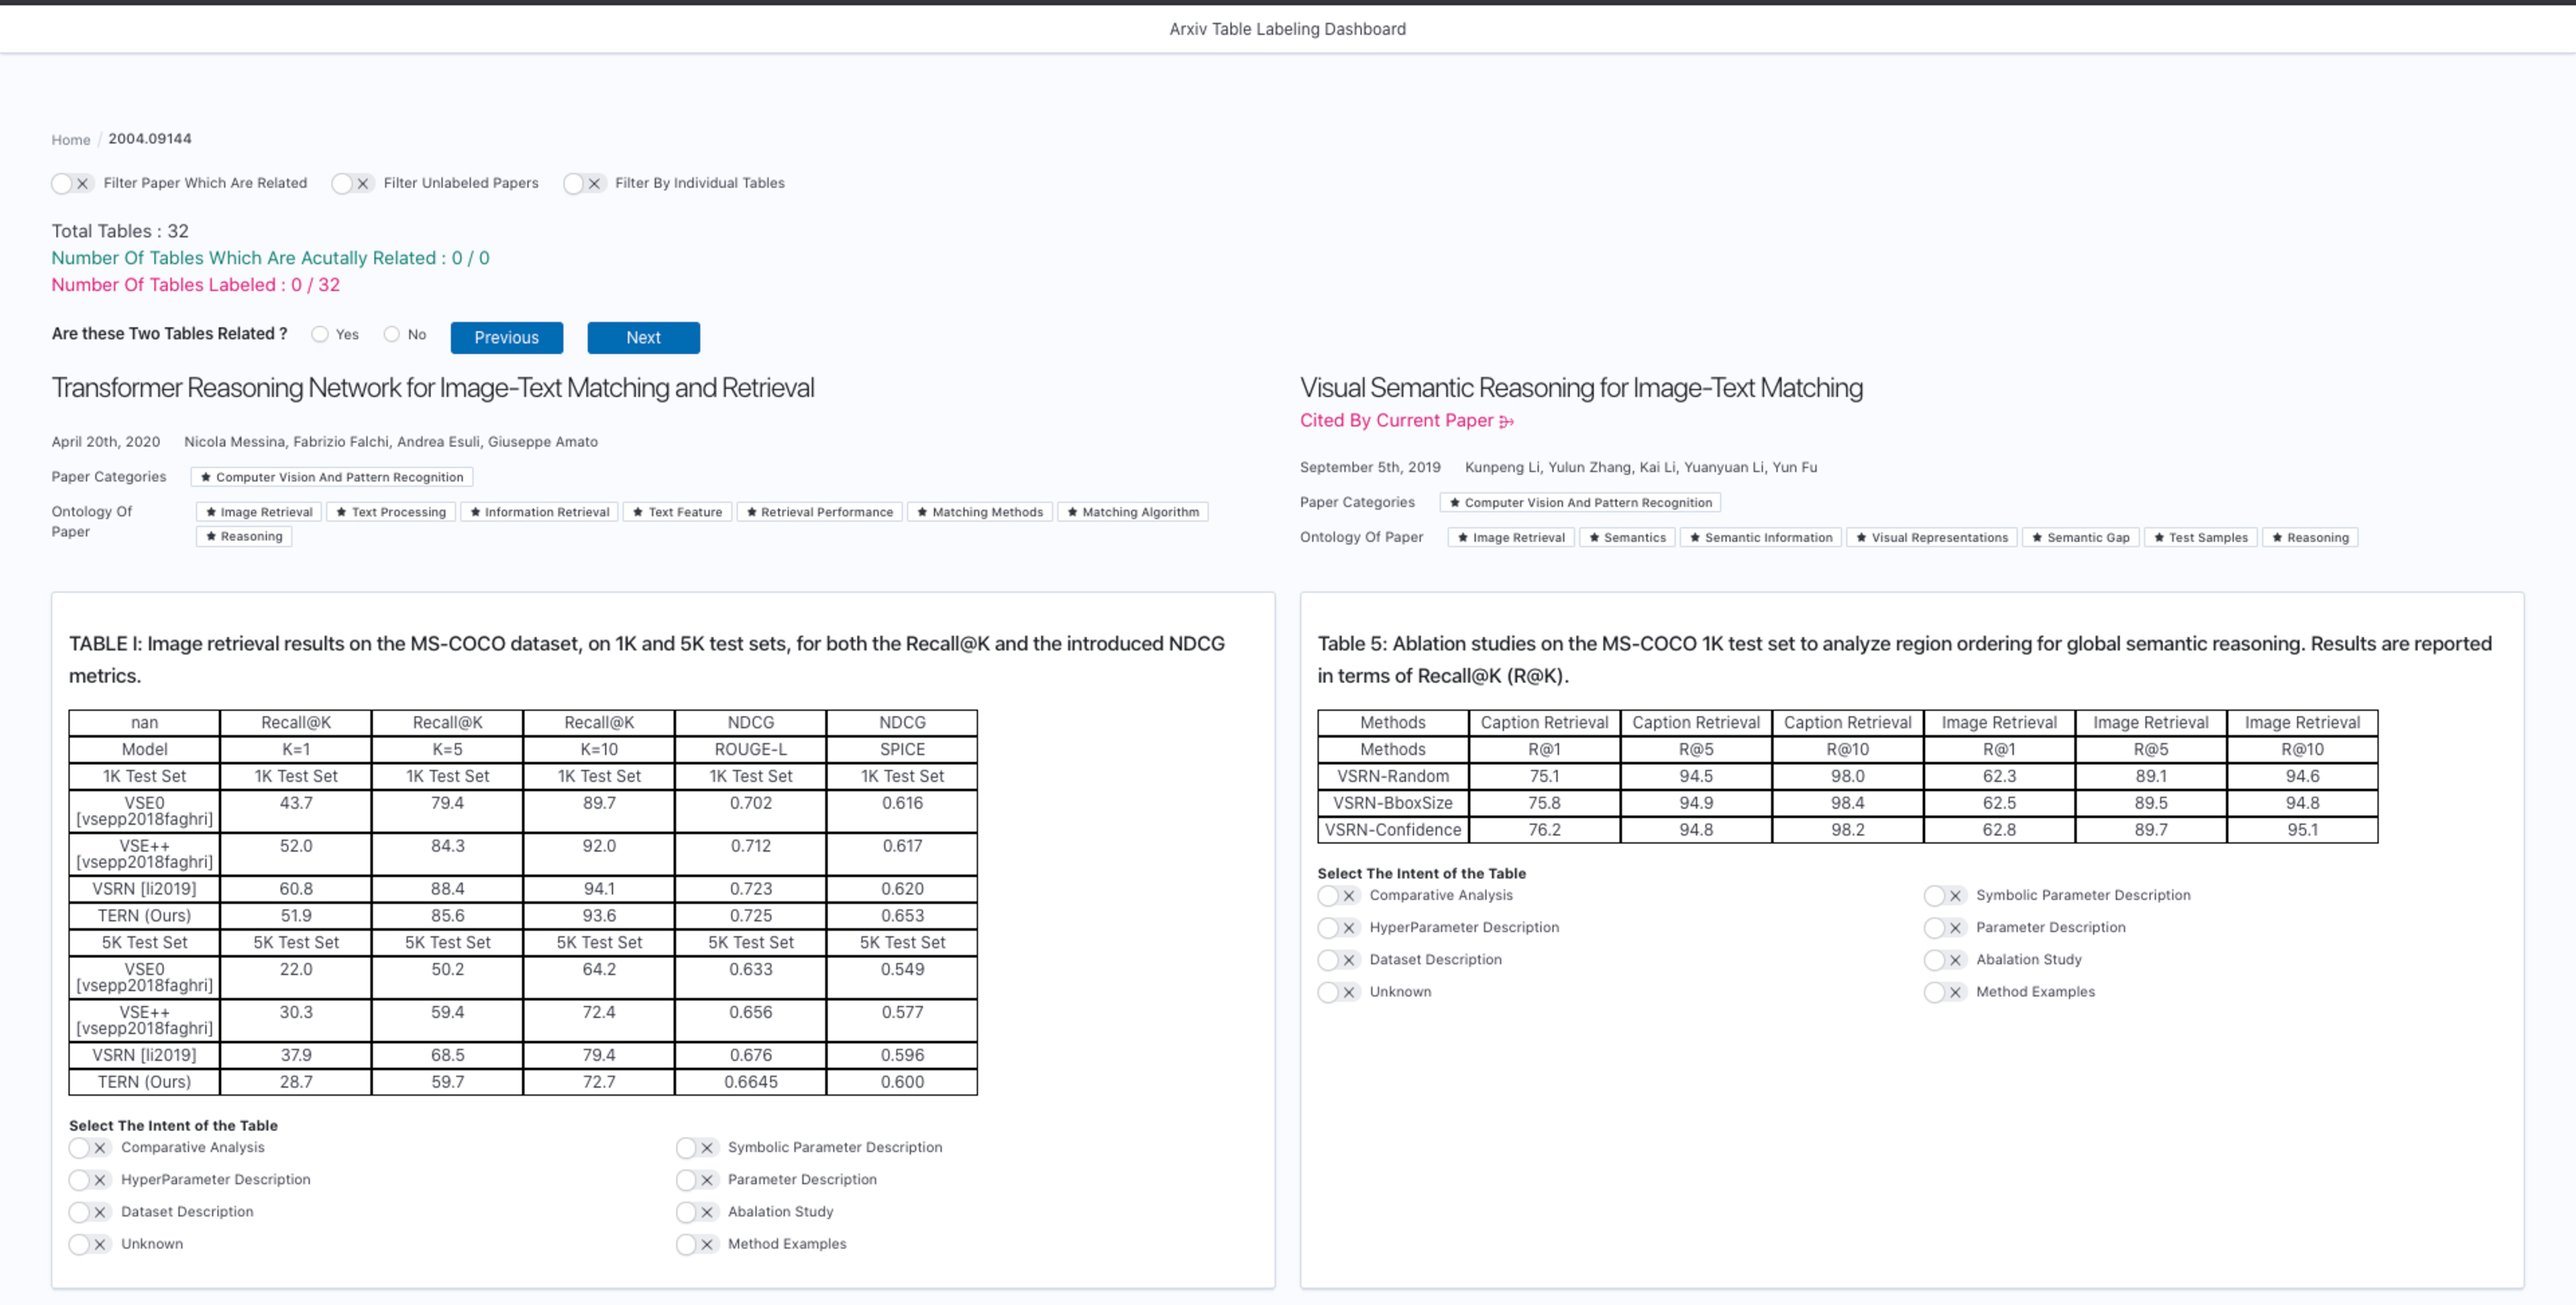
\includegraphics[width=\maxwidth{\textwidth}]{src/images/table-lable-exp.pdf}
    \caption{Table Labeling Interface For Table Relation and Intent Annotation}
    \label{figure\arabic{figurecounter}}
\end{figure}
\refstepcounter{figurecounter}

As Sci-Genie consists of a Data Layer (Chapter \ref{sci-genie-core:data-layer}) that contains the tables from the research papers, A labeling interface(Figure \ref{figure16}) is designed to annotate tables from 240 research papers. 820 tables are annotated out of which 574 tables are describing a comparison and 246 are not. The labeling interface supports labeling types to tables described by \cite{kim2012scientific} and few more based on the observations from current CS research. More details regarding this subject are discussed in Chapter \ref{conclusion:future-scope:type-class}. 

\section{Experiment Results}
\label{table_classification:experiement-result}
\begin{figure}[h]
    \centering
    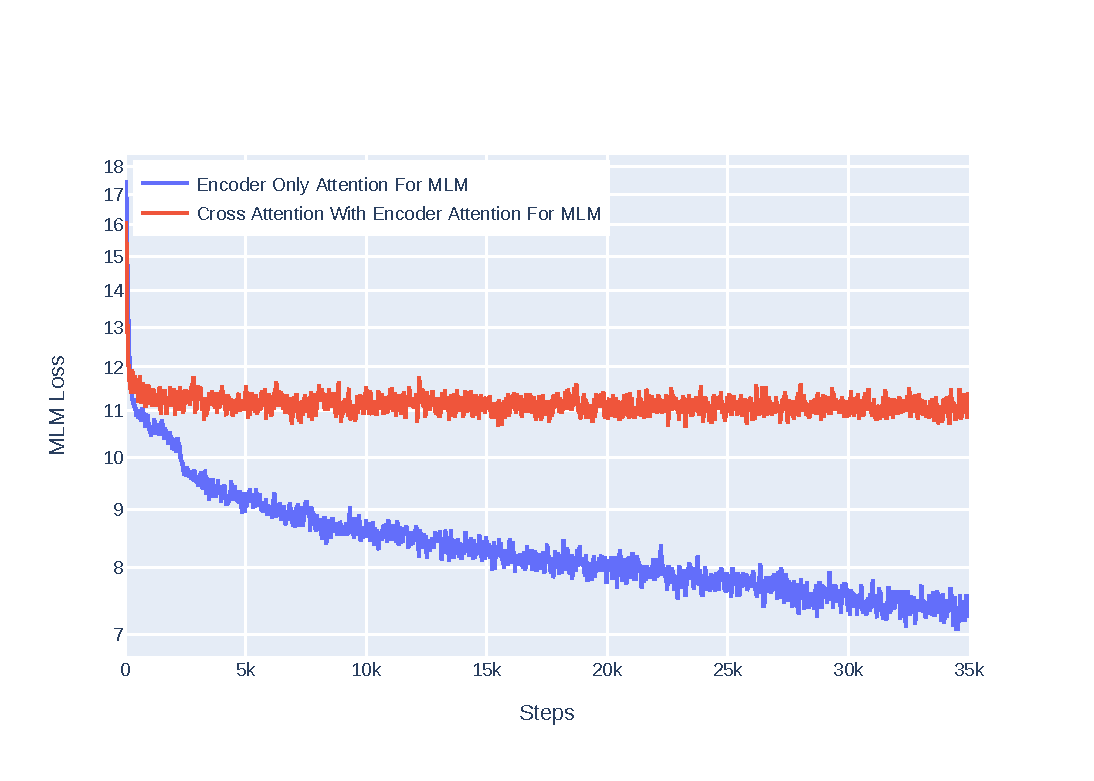
\includegraphics[width=\maxwidth{\textwidth}]{src/images/mlm-loss-comparison.pdf}
    \caption{Masked Language Modeling(MLM) Loss For Encoder Style Attention VS Cross Attention. The MLM losses for $T$ and $C$ are summed}
    \label{figure\arabic{figurecounter}}
\end{figure}
\refstepcounter{figurecounter}

\begin{table}[h]
    \label{table\arabic{tablecounter}}
    \centering
    \begin{tabular}{|p{4cm}|p{3cm}|p{3cm}|p{3cm}|}
    \hline
        \textbf{Model} & \textbf{Accuracy} (\%) & \textbf{F1 Score}  & \textbf{Loss} \\ \hline
        Naive Bayes & 71.6 & 0.825 & - \\ \hline
        SVM  & 78.39 & 0.85477 & - \\ \hline
        Cross Channel Transformer From Scratch (31M) & $73.95 \pm 10.5 $ & $0.739 \pm 0.107$ & $0.53 \pm 0.08$ \\ \hline
        Encoder Only Multi-Channel Pretained (25M) & $88.33 \pm 0.29$ & $0.8883 \pm 0.002$ & $0.423 \pm 0.007$ \\ \hline
        Cross Channel Transformer Pretained (31M) & $87.5 \pm 1.8$ & $0.875 \pm 0.018$ & $0.34 \pm 0.016$ \\ \hline
        SciBert Finetuned (112M) & $92.23 \pm 1.60$ & $0.923 \pm 0.016$ & $0.21 \pm 0.04$ \\ \hline
    \end{tabular}
    \caption{\label{tablecounter} Test set results of the table classification models using SOTA Transformer and baselines. Average Results from 4 Training runs is reported}
\end{table}
\refstepcounter{tablecounter}
The following are the experiment and their conditions for ML model training:
\begin{itemize}
    \item Cross Channel Transformer: Pretrained with 70K Tables and finetuned on the classification task
    \item Cross Channel Transformer: Directly trained from scratch on the classification task 
    \item Encoder Only Multi-Channel Transformer : Pretrained with 70K Tables and finetuned on the classification task
    \item SciBert: Finetuned on the classification task.
    \item Naive Bayes \& SVM
\end{itemize}
More details on the hyperparameters for the experiments are found in the Appendix \ref{appendix:toc}. All experiments are conducted on the same frozen test set with evenly balanced samples. Numbers are reported after averaging 4 training runs.

All experiments are conducted using Google Colab Notebooks on NVIDIA P100 GPUs. Table \ref{table5} describes the results of the experiments. 

The pretrained models perform substantially better than the baselines. The Cross-Channel Tranformer when pretrained from scratch performs substantially better than the model trained from scratch. The Encoder Only Multi-Channel Transformer performs the best among all the models pretrained on ArXiv Tables. SciBert outperforms all models. The reason for Sci-Bert's better performance can be inferred based on the study by \cite{hernandez2021scaling}. As SciBert is a much bigger model, trained on a very large corpus consisting of data from a similar distribution, its performance would be better than the baseline and the developed models. It can also be seen from Table \ref{table5} that pretraining has a direct influence on a better model compared to training the model from scratch. 